\documentclass{article}
\usepackage[utf8]{inputenc}
\usepackage{indentfirst}
\usepackage{titling}
\usepackage{geometry}
\usepackage{graphicx}
\graphicspath{ {./Images/} }
\usepackage[shortlabels]{enumitem}
\usepackage{fancyhdr}
\usepackage{ulem}
\usepackage[dvipsnames]{xcolor}
\usepackage{amssymb}

\def\ojoin{\setbox0=\hbox{$\bowtie$}%
  \rule[-.02ex]{.25em}{.4pt}\llap{\rule[\ht0]{.25em}{.4pt}}}
\def\leftouterjoin{\mathbin{\ojoin\mkern-5.8mu\bowtie}}
\def\rightouterjoin{\mathbin{\bowtie\mkern-5.8mu\ojoin}}
\def\fullouterjoin{\mathbin{\ojoin\mkern-5.8mu\bowtie\mkern-5.8mu\ojoin}}

\renewcommand\maketitlehooka{\null\mbox{}\vfill} %para centralizar verticalmente
\renewcommand\maketitlehookd{\vfill\null}
\pagestyle{fancy}
\fancyhf{}
\rfoot{\thepage}
\lfoot{ 
\includegraphics[scale=0.01]{UA.jpg} José Mendes 107188 LEI}
\geometry{
  a4paper,
  headheight=4cm,
  top=5.5cm,
  bottom=4.5cm,
  footskip=4cm
}


\title{Tecnologias e Programação Web}
\author{José Mendes 107188}
\date{2023/2024}

\begin{document}


\begin{titlepage}
    \maketitle
    \begin{center}
        
\includegraphics[scale=0.4]{UA.png}
    \end{center}
    \thispagestyle{empty} %remove o count da pagina
\end{titlepage}

\pagebreak
%depois por um index aqui

\section{Arquiteturas de Aplicações Web}

\subsection{Independência dos Dados nas Bases de Dados}

\subsubsection{Arquitetura da Base de Dados e Views}

\begin{center}
    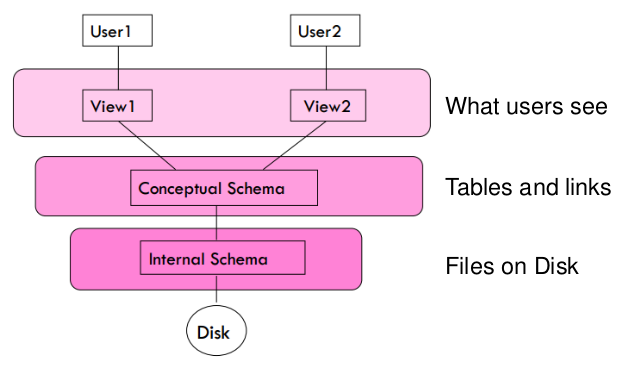
\includegraphics[scale=0.4]{1}
\end{center}

\subsubsection{Independência Lógica e Física}

\begin{center}
    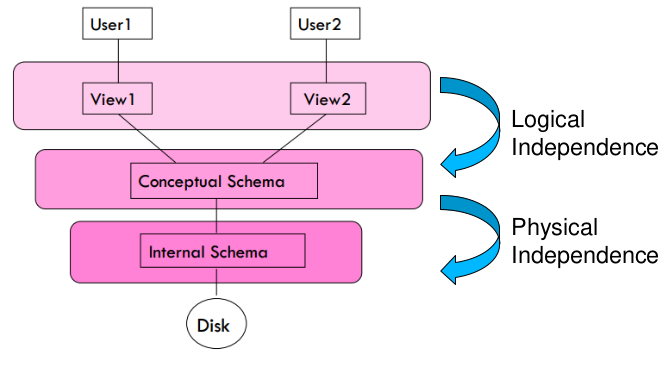
\includegraphics[scale=0.4]{2}
\end{center}

\begin{flushleft}
  Cada nível é independente dos níveis a baixo.
\end{flushleft}

\pagebreak

\subsubsection{Independência dos Dados}

\begin{flushleft}
  \textbf{Independência Física:} Capacidade de alterar o schema interno sem alterar
  o schema conceptual.
  \begin{itemize}
    \item Espaço de armazenamento pode mudar;
    \item O tipo de alguns dados pode mudar por razões de eficiência/otimização;
  \end{itemize}

  \textbf{Independência Lógica:} Capacidade de alterar o schema conceptual sem alterar
  as Views ou os programas de aplicação.
  \begin{itemize}
    \item Pode adicionar novos campos, novas tabelas sem alterar as Views;
    \item Pode alterar a estrutura das tabelas sem alterar as Views;
  \end{itemize}

  \vspace{5mm}

  \textbf{Nota:} Manter a \textbf{View} (aquilo que o user vê) \uline{independente} do \textbf{Modelo} (domain knowledge).
\end{flushleft}

\subsection{Arquiteturas N-Tier}

\subsubsection{Significado de "Tiers"}

\begin{flushleft}
  Arquiteturas N-Tier têm as mesmas camadas:
  \begin{itemize}
    \item \textbf{Presentation Tier:} Camada de apresentação;
    \item \textbf{Business/Logic Tier:} Camada de lógica/de negócio;
    \item \textbf{Data Tier:} Camada de dados;
  \end{itemize}

  Arquiteturas N-Tier tentam separar as camadas em diferentes tiers.
  \begin{itemize}
    \item \textbf{Camada}: Separação lógica;
    \item \textbf{Tier}: Separação física;
  \end{itemize}
\end{flushleft}

\subsubsection{Arquitetura 1-Tier}

\begin{center}
  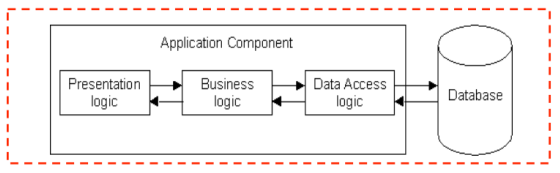
\includegraphics[scale=0.4]{3}
\end{center}

\begin{flushleft}
  As 3 camadas estão no mesmo computador (máquina). Isto é, todo o código e processamento
  está numa única máquina.

  As camadas de apresentação, lógica e de dados estão firmemente conectados.
  \begin{itemize}
    \item \textbf{Escalabilidade:} Um único processador implica que é díficil de
    aumentar o volume de processamento;
    \item \textbf{Portabilidade:} Mudar para outro computador pode implicar
    reescrever tudo;
    \item \textbf{Manutenção:} Mudar uma camada requer mudar outras camadas;
  \end{itemize}
\end{flushleft}


\subsubsection{Arquitetura 2-Tier}

\begin{center}
  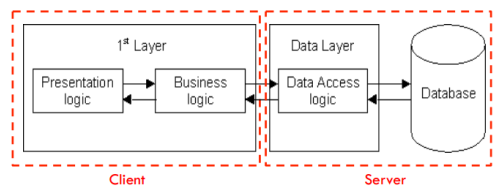
\includegraphics[scale=0.4]{4}
\end{center}

\begin{flushleft}
  A base de dados corre no servidor, separado do cliente, sendo fácil de
  mudar para uma base de dados diferente.

  As camadas de apresentação e lógica ainda estão firmemente conectados.
  \begin{itemize}
    \item Carga pesada no servidor;
    \item Potencial congestionamento da rede;
    \item Apresentação ainda está firmemente conectada à lógica de negócio;
  \end{itemize}
\end{flushleft}

\subsubsection{Arquitetura 3-Tier}

\begin{center}
  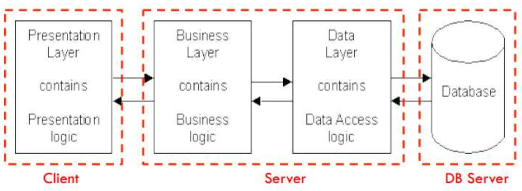
\includegraphics[scale=0.4]{5}
\end{center}

\begin{flushleft}
  Cada camada pode, potencialmente, correr numa máquina diferente.
  As camadas de apresentação, lógica e de dados estão disconectadas. 
\end{flushleft}

\begin{flushleft}
  \textbf{Típica Arquitetura 3-Tier}
\end{flushleft}

\vspace{5mm}

\begin{center}
  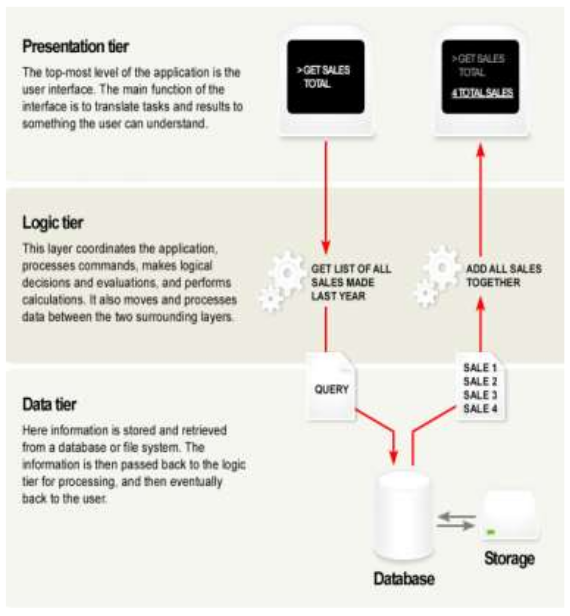
\includegraphics[scale=0.3]{6}
\end{center}


\pagebreak

\begin{flushleft}
  \textbf{Princípios de Arquitetura:}
  \begin{itemize}
    \item Arquitetura \textbf{Cliente-Servidor};
    \item Cada camada (Apresentação, Lógica, Dados) deve ser independente e não deve
    expôr dependências relacionadas com a implementação;
    \item Camadas disconectadas não devem comunicar;
    \item Alterações numa plataforma afetam apenas a camada que corre que essa plataforma;
  \end{itemize}

  \textbf{Camada de Apresentação:}
  \begin{itemize}
    \item Fornece a interface do utilizador;
    \item Lida com a interação com o utilizador;
    \item Por vezes chamada de GUI, client view ou \textbf{front-end};
    \item Não deve conter lógica de negócio ou código de acesso aos dados;
  \end{itemize}

  \textbf{Camada de Lógica:}
  \begin{itemize}
    \item O conjunto de regras para processar a informação;
    \item Pode acomodar vários utilizadores;
    \item Por vezes chamada de \textbf{middleware} ou back-end;
    \item Não deve conter apresentação ou código de acesso aos dados;
  \end{itemize}

  \textbf{Camada de Dados:}
  \begin{itemize}
    \item A camada de armazenamento físico, para persistir os dados;
    \item Gere o acesso à base de dados ou sistema de ficheiros;
    \item Por vezes chamada de \textbf{back-end};
    \item Não deve conter apresentação ou código da lógica de negócio;
  \end{itemize}
\end{flushleft}

\subsubsection{Arquitetura 3-Tier para Aplicações Web}

\begin{flushleft}
  \textbf{Camada de Apresentação:} Conteúdo estático ou dinâmico, renderizado pelo browser (\textbf{front-end});
  
  \textbf{Camada de Lógica:} Processamento de conteúdo dinâmico, geração de servidores de aplicação
  (e.g. Java EE, ASP.NET, Python Django Framework) (\textbf{middleware});
  
  \textbf{Camada de Dados:} Base de dados, composta por ambos, conjunto dos dados e o sistema de gestão de base de dados
  ou software RDBMS que gere e fornece acesso aos dados (\textbf{back-end});
\end{flushleft}

\pagebreak

\subsubsection{Arquitetura 3-Tier - Vantagens}

\begin{flushleft}
  \textbf{Independência das camadas}
  \begin{itemize}
    \item Mais fácil de manter;
    \item Componentes são reutilizáveis;
    \item Desenvolvimento mais rápido (divisão do trabalho, 
    Web Designer faz a apresentação, Engenheiros de Software fazem a lógica
    e administradoes de base de dados fazem o modelo de dados);
  \end{itemize}
\end{flushleft}

\subsection{Padrões de Desenho}

\subsubsection{Padrões de Desenho e Decisões}

\begin{flushleft}
  \begin{itemize}
    \item Contrução e teste;
    \begin{itemize}
      \item como contruímos uma aplicação web?
      \item que tecnologias devemos escolher?
    \end{itemize}

    \item Reutilizar;
    \begin{itemize}
      \item podemos usar componentes normais?
    \end{itemize}

    \item Escalabilidade;
    \begin{itemize}
      \item como vai a nossa aplicação web lidar com um elevado número de pedidos?
    \end{itemize}

    \item Segurança;
    \begin{itemize}
      \item como proteger contra um attack, vírus, acesso malicioso dos dados, denial of service?
    \end{itemize}


    \item Diferentes views de dados;
    \begin{itemize}
      \item tipos de users, contas individuais, proteção de dados
    \end{itemize}
  \end{itemize}

  \vspace{5mm}
  \textbf{Nota:} Precisamos de uma solução geral e reutilizável: \textbf{Padrões de Desenho}
\end{flushleft}

\subsubsection{O que é um Padrão de Desenho?}

\begin{flushleft}
  Uma solução geral e reutilizável para um problema recorrente no desenho de software.
  É um template para como resolver um problema que tenha sido usado em várias situções diferentes.

  \textbf{NÂO} é um design completo, o padrão precisa de ser adaptado à aplicação,
  não podemos simplesmente traduzir o padrão para código.
\end{flushleft}

\pagebreak

\subsubsection{Origem do Padrão de Desenho}

\begin{flushleft}
  \begin{itemize}
  \item Arquitetura conceptual por Christopher Alexander (1977/1979).
  \item Adaptado para programação OO por Kent Beck e Ward Cunningham (1987).
  \item Ganhou popularidade em CS com o livro "Design Patterns: Elements of Re-usable Object-Oriented Software" (1994),
  por Erich Gamma, Richard Helm, Ralph Johnson e John Vlissides (Gang of Four).
  \item Agora bastante utilizado em Engenheiria de Software.
  \end{itemize}
\end{flushleft}

\subsection{O Padrão de Desenho MVC}

\subsubsection{O Problema do Desenho}

\begin{flushleft}
  \begin{itemize}
    \item Preciso mudar o look-and-feel sem mudar o core/logic;
    \item Preciso de apresentar os mesmos dados de diferentes formas (e.g. computadores bons, web, dispositivos móveis);
    \item Preciso de interagir/acessar os dados de diferentes formas (e.g. ecrã tátil nos dispositivos móveis, teclado no computador);
    \item Preciso de manter várias views para a mesma informação (e.g lista, thumbnails, detalhes, \dots);
  \end{itemize}
\end{flushleft}

\subsubsection{A Solução do Desenho}

\begin{flushleft}
  \begin{itemize}
    \item Separar a funcionalidade chave da apresentação e lógica que usa esta funcionalidade;
    \item Permitir múltiplas views para partilhar o mesmo modelo de dados;
    \item Tornar o suporte de vários clientes mais fácil de implementar, testar e manter;
  \end{itemize}
\end{flushleft}

\subsubsection{O Padrão Model-View-Controller}

\vspace{3mm}

\begin{center}
  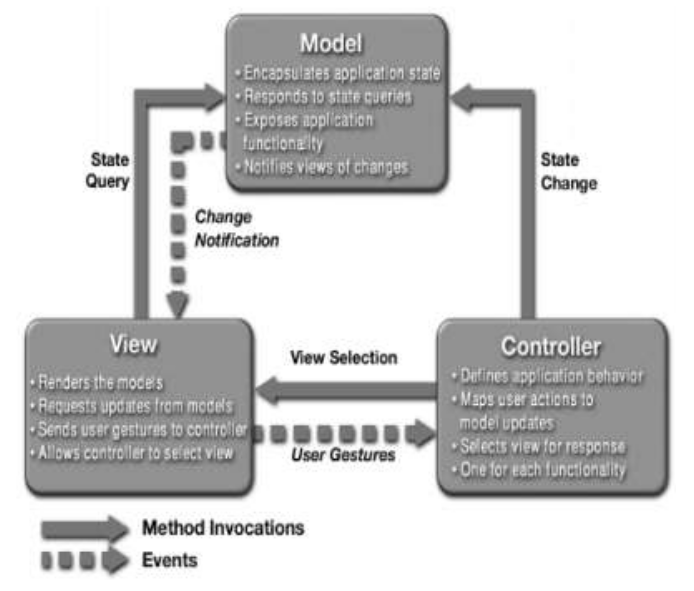
\includegraphics[scale=0.3]{7}
\end{center}

\pagebreak

\begin{flushleft}
  Padrão de Desenho para sistemas gráficos que \textbf{promove a separação entre o modelo e a view}.
  Com este padrão, a lógica necessária para manutenção dos dados (base de dados, ficheiro de texto),
  \textbf{é separada} de como os dados são apresentados (gráfico, numerico) e como
  os dados são manipulados (GUI, linha de comandos, touch).
\end{flushleft}

\begin{flushleft}
  \textbf{Model}
  \begin{itemize}
    \item Gere o comportamento e os dados do domínio da aplicação;
    \item Responde a pedidos por informação sobre o estado (normalmente da view),
    segue instruções para alterar o estado (normalmente do controller);
  \end{itemize}

  \textbf{View}
  \begin{itemize}
    \item Renderiza o modelo para uma forma apropriada para a interação,
    tipicamente uma interface do utilizador (várias views podem existir para o mesmo modelo
    com diferentes intenções);
  \end{itemize}

  \textbf{Controller}
  \begin{itemize}
    \item Recebe os inputs e inicia uma resposta realizando chamadas em objetos do modelo;
    \item Aceita input do utilizador e intrui o modelo e a view para realizar ações baseadas no input;
  \end{itemize}
\end{flushleft}


\subsubsection{O Padrão MVC na prática}

\begin{flushleft}
  \textbf{Model}
  \begin{itemize}
    \item Contém conhecimento específico do domínio;
    \item Regista o estado da aplicação (e.g quais items estão no carrinho de compras);
    \item Normalmente conectado com a base de dados;
    \item Independente da view (um model pode ter várias views);
  \end{itemize}

  \textbf{View}
  \begin{itemize}
    \item Apresenta dados ao utilizador;
    \item Permite interação com o utilizador;
    \item Não faz processamento;
  \end{itemize}
    
  \textbf{Controller}
  \begin{itemize}
    \item Define como a interface do utilizador reage a inputs (eventos);
    \item Recebe mensagens da view (de onde os eventos vêm);
    \item Envia mensagens ao modelo (diz quais dados mostrar)
  \end{itemize}
\end{flushleft}

\pagebreak

\subsubsection{O MVC para Aplicações Web}

\begin{flushleft}
  \textbf{Model}
  \begin{itemize}
    \item Tabelas da base de dados (dados persistentes);
    \item Informações sobre a sessão (dados atuais do sistema de dados)
    \item Regras sobre transações;
  \end{itemize}

  \textbf{View}
  \begin{itemize}
    \item (X)HTML;
    \item CSS style sheets;
    \item Templates server-side;
  \end{itemize}

  \textbf{Controller}
  \begin{itemize}
    \item Scripts client-side;
    \item Processamento de pedidos HTTP;
    \item Lógica de negócio/preprocessamento;
  \end{itemize}
\end{flushleft}

\subsubsection{MVC - Vantagens}

\begin{flushleft}
  \textbf{Clareza de Design}
  \begin{itemize}
    \item métodos do modelo dão uma API para os dados e o estado;
    \item o design da view e do controller são fáceis; 
  \end{itemize}

  \textbf{Modularidade eficiente}
  \begin{itemize}
    \item qualquer componente pode ser facilmente substituído;
  \end{itemize}

  \textbf{Várias views}
  \begin{itemize}
    \item Várias views podem ser criadas conforme apropriado;
    \item Cada uma usa a mesma API para o modelo;
  \end{itemize}

  \textbf{Mais fácil de contruir e manter}
  \begin{itemize}
    \item Views simples (baseado em texto) durante o desenvolvimento (contrução);
    \item Mais views e controllers podem ser adicionados mais tarde;
    \item Fácil de contruir interfaces estáveis;
  \end{itemize}

  \textbf{Distribuível}
  \begin{itemize}
    \item Ajuste natural para ambientes distribuídos;
  \end{itemize}
\end{flushleft}

\pagebreak

\subsubsection{3-Tier Architecture vs Padrão MVC}

\begin{flushleft}
  \begin{itemize}
    \item Comunicação
    \begin{itemize}
      \item \textbf{3-Tier:} A camada de apresentação nunca comunica diretamente
      com a camada de dados, apenas através da camada de lógica (topologia linear);
      \item \textbf{MVC:} Todas as camadas comunicam diretamente (topologia triangular);
    \end{itemize}

    \item Usabilidade
    \begin{itemize}
      \item \textbf{3-Tier:} É usada em aplicações web onde os tiers cliente, middleware
      e os dados corram em plataformas fisicamente separadas;
      \item \textbf{MVC:} Historicamente usada em aplicações que correm numa única estação de trabalho gráfica;
      \begin{itemize}
        \item No contexto de aplicações web, contudo, os componentes lógicos podem ser
        desacoplados para cumprir com uma verdadeira arquitetura 3-Tier;
      \end{itemize}
    \end{itemize}
  \end{itemize}
\end{flushleft}

\section{Introdução à Plataforma Django}

\subsection{Introdução}

\begin{flushleft}
  \textbf{Django} é uma plataforma gratuita e open-sourc, escrita em Python,
  para o desenvolvimento de aplicações web.
  Tem o nome do famoso guitarrista de jazz Django Reinhardt.
  É mantida pela Django Software Foundation (DSF), uma organização independente.
  Fomenta o desenvolvimento rápido, limpo e pragmático.
  Criada em 2003, lançada open-source em 2005.
\end{flushleft}

\subsection{Características}

\begin{flushleft}
  \begin{itemize}
    \item Segue, parcialmente, o padrão MVC;
    \item Possuuie um ORM (Object-Relational Mapper) para processar dados;
    \item Focada na automatização, aderinco ao princípio DRY (Don't Repeat Yourself);
    \item Usa um sistema de templates;
    \item Sistema de personalização Admin, para facilitar o CRUD;
    \item Desenho elegante de routing de URLs;
    \item Possui um light web server embotido (para testes);
    \item Possibilita a utilização de moddleware personalizado;
    \item Possui facilidades para: autenticação, internacionalização, caching;
  \end{itemize}
\end{flushleft}

\pagebreak

\subsection{Arquitetura}

\begin{center}
  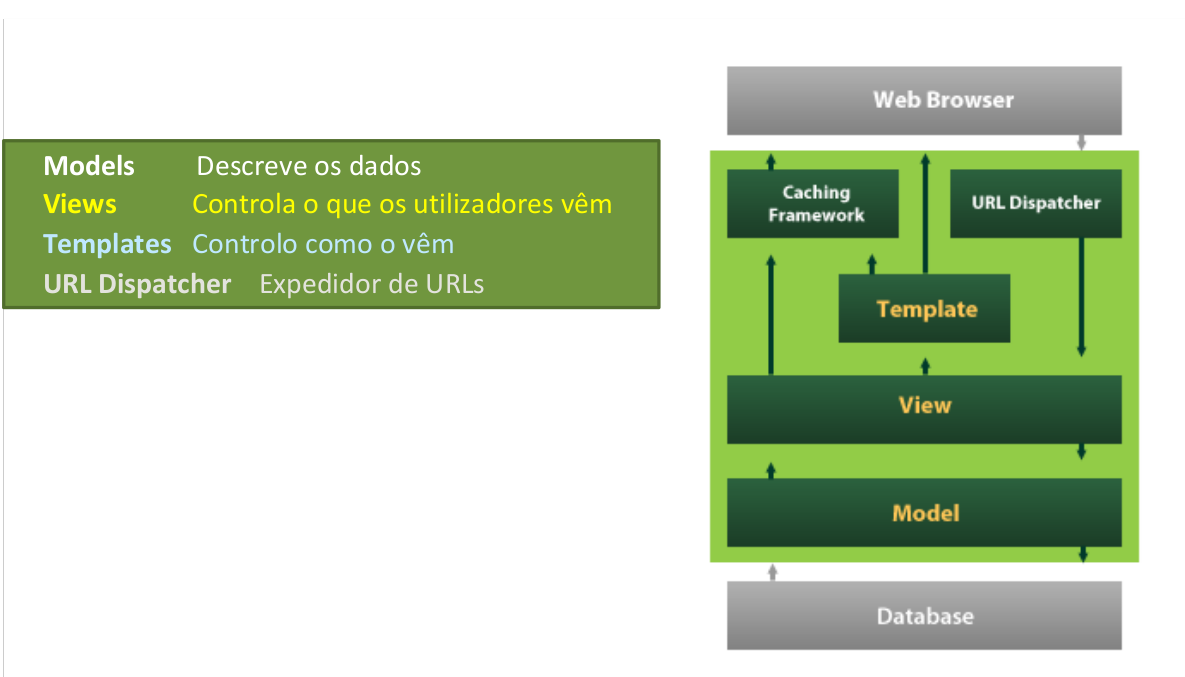
\includegraphics[scale=0.3]{8}
\end{center}

\subsection{Estrutura de um Projeto Django}

\begin{center}
  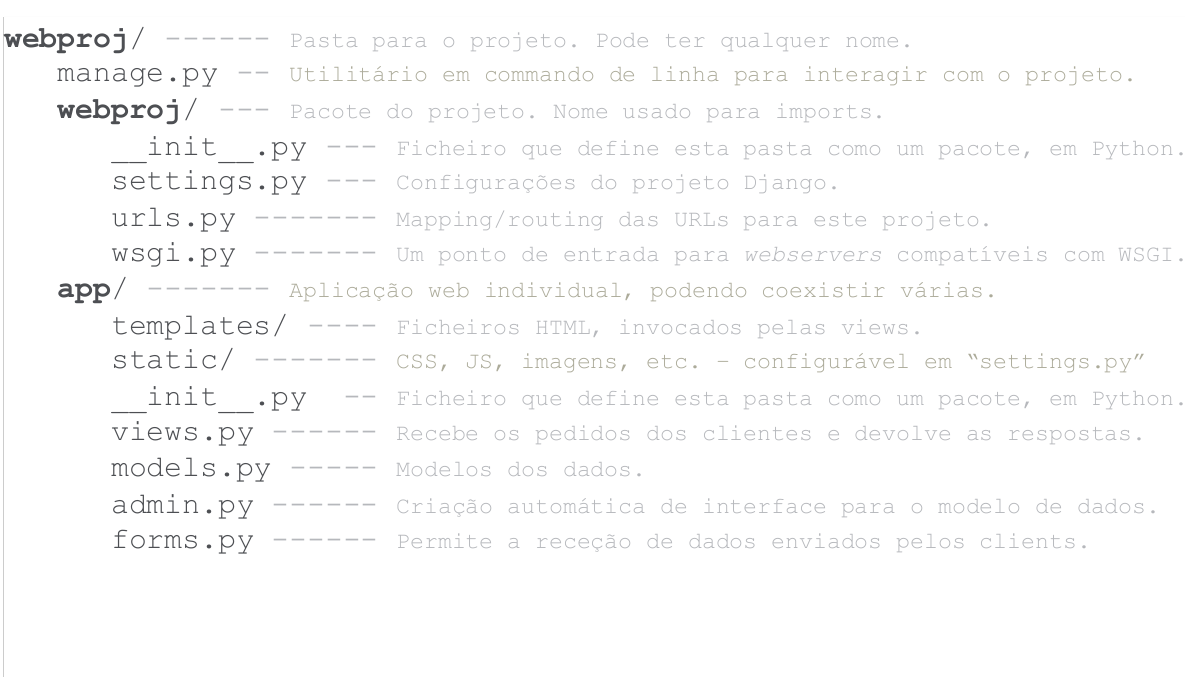
\includegraphics[scale=0.3]{9}
\end{center}

\pagebreak

\subsection{Settings}

\begin{flushleft}
  Possui um ficheiro de configuração, \textbf{settings.py},
  do projeto Django, sobrepõe as configurações padrão
  (ficheiro <python>/lib/sitepackages/django/conf/global\_settings.py).

  \vspace{2mm}
  Possui alguns atributos como: \textbf{DEBUG} (True/False),
  \textbf{DATABASES ENGINES} (sqlite3, mysql, postgresql, oracle),
  \textbf{ROOT\_URLCONF} (nome do ficheiro de routing de URLs),
  \textbf{MEDIA\_ROOT} (para ficheiros enviados pelo utilizador),
  \textbf{MEDIA\_URL} (para ficheiros multimédia),
  \textbf{STATIC\_ROOT} (pasta para ficheiros estáticos, CSS, JS),
  \textbf{STATIC\_URL} (pasta de ficheiros estáticos),
  \textbf{TEMPLATE\_DIRS} (pasta de templates)
\end{flushleft}

\subsection{Criação de um Projeto Django}

\begin{flushleft}
  Nesta cadeira vamos usar o PyCharm, pelo que para criar um projeto Django
  basta selecionar a opção \textbf{Django} e chamar a pasta dos templates de
  \textbf{app/templates} e a pasta da aplicação de \textbf{app}.
  
  Para correr basta clicar em Run e aceder ao link \textbf{http://127.0.0.1:8000}.

  Ou podemos usar o comando \textbf{python manage.py runserver}.
\end{flushleft}

\subsubsection{Views}

\begin{flushleft}
  No ficheiro "app/views.py"  podemos inserir views:
\end{flushleft}

\begin{center}
  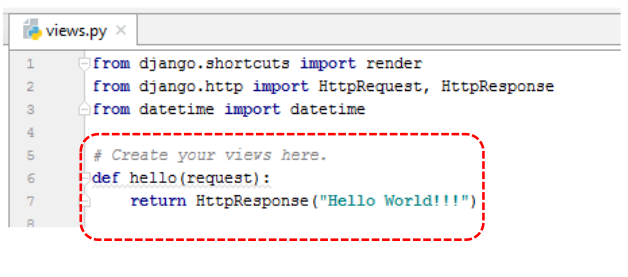
\includegraphics[scale=0.3]{10}
\end{center}

\begin{flushleft}
  Para criar uma nova, basta criar uma nova view function.
\end{flushleft}

\subsubsection{Configuração da URL}

\begin{flushleft}
  No ficheiro "nome\_do\_projeto/urls.py" podemos configurar as URLs:
\end{flushleft}

\begin{center}
  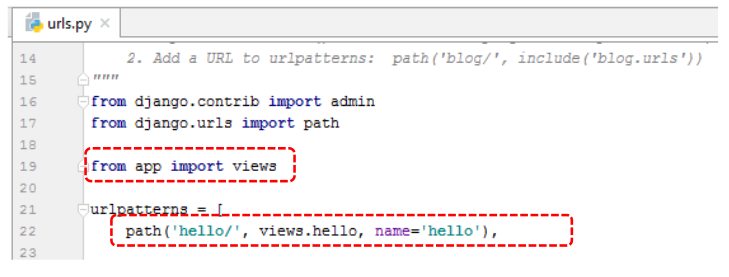
\includegraphics[scale=0.3]{11}
\end{center}

\begin{flushleft}
  Para criar uma nova, basta inserir mais uma route para a view.
\end{flushleft}

\subsubsection{Templates}

\begin{flushleft}
  Podemos usar variáveis usando \{\{ var\_name \}\} e template tags (como if)
  usando \{\% if \dots \%\}.
\end{flushleft}

\pagebreak

\subsubsection{Ficheiros estáticos}

\begin{flushleft}
  São ficheiros que se pretende simplesmente referenciar e servir ao cliente,
  sem qualquer processamento prévio.

  O seu acesso é público, pois o cliente apenas necessita do URL para os mesmos.

  Exemplos:
  \begin{itemize}
    \item Imagens (jpg, png, gif, \dots);
    \item Style Sheets (CSS);
    \item Scripts (JavaScript);
    \item \dots
  \end{itemize}
\end{flushleft}

\subsubsection*{Localização}

\begin{flushleft}
Os ficheiros denominados por static files
residem em pastas pré-determinadas, dentro
ou fora da “app” (normalmente uma pasta denominada de "static").
\end{flushleft}

\subsubsection*{Configuração}

\begin{flushleft}
  No ficheiro "settings.py" podemos configurar os ficheiros estáticos:
  \begin{enumerate}
    \item o módulo 'django.contrib.staticfiles' deve aparecer
    nas aplicações instaladas “INSTALLED\_APPS”
    \item o atributo STATIC\_URL deve ser definido (ex: '/static/')
    \item a pasta dos static files deve estar definida no atributo STATIC\_ROOT
    (ex: os.path.join(BASE\_DIR, 'app/static'))
  \end{enumerate}
\end{flushleft}

\subsubsection*{Uso}

\begin{flushleft}
  Para usar basta usar a tag \{\% load static \%\} e depois
  referenciar o ficheiro.
\end{flushleft}

\end{document}